\chapter{研究$J/\psi$的极化及其影响}%
\section{简介}
只有深刻的认识到$J/\psi$的状态才能更深一步的研究其衰变性质
。正负电子对产生的$J/\psi$
与正负质子对、质子对撞、$B_{s}$衰变、$\psi(2S)$衰变、$\chi_{cJ}$衰变的极化状态截然不同,
% https://arxiv.org/pdf/1909.03370.pdf B_{s} -> phi J/psi
其中最重要的差别是$J/psi$的极化状态不同。这一节是研究超子对产生性质的前奏。在下面的小
节中,将首先论述正负电子对产生的$J/\psi$的极化状态,接着以$J/\psi \to e^{+} e^{-} P$为例
说明极化状态对实验测量的影响,并对其分支比进行了预言。
\subsection{$\psi$的极化状态}
在这一章节中,我们将研究正负电子对撞机产生的$J/\psi$极化状态。一般的,有质量的矢量粒子有三种极化状态,它们分别是:
\begin{equation}
  \begin{split}
    \epsilon^{\mu}_{\rm{LP}} &= (0,0,0,1) \\ 
    \epsilon^{\mu}_{\rm{TL}} &= \frac{1}{\sqrt{2}}(0,1,-i,0) \\ 
    \epsilon^{\mu}_{\rm{TR}} &= \frac{1}{\sqrt{2}}(0,1,i,0)
  \end{split}
\end{equation}
式中的$\epsilon^{\mu}_{\rm{LP}}$,  $\epsilon^{\mu}_{\rm{TL}}$ 及 $\epsilon^{\mu}_{\rm{TR}}$分别
代表纵向极化,左旋及右旋极化状态。

考虑到洛伦茨不变性及宇称守恒过程$e^{+} e^{-} \to \psi$的振幅的一般形式为 
\begin{equation}
    T = e_{c} e f_{\psi} \frac{m_{\psi}}{q^{2}} 
    \bar{u}(k_{1}) \gamma_{\mu} \nu(k_{2}) \epsilon^{\mu}
\end{equation}
式中$e_{c}$和$e$分别是$c$夸克和电子电荷,$m_{\psi}$为$\psi$介子的质量,$k_{1}$ ($k_{2}$)是
电子(反电子)的动量,$\epsilon^{\mu}$是$\psi$的极化矢量。
很容易得到$|T|^{2}$为:
\begin{equation}
\begin{split}
|T(\psi)|^{2} =  & \frac{16\pi^{2}\alpha^{2}e^{2}_{c}}{q^{4}}|f_{\psi}|^{2}m^{2}_{\psi}\epsilon^{*}_{\mu}\epsilon_{\nu} \\ & \times (k^{\mu}_{1}k^{\nu}_{2} + k^{\mu}_{2}k^{\nu}_{1} - g^{\mu\nu}k_{1}\cdot k_{2} + g^{\mu\nu}m^{2}_{e}),
\end{split}
\end{equation}
式中的$m$为电子的质量,$q=k_{1}+k_{2}$。
经过简单的计算可以得到三种极化状态的相对比例为:
\begin{equation}
\begin{split}
|T( \psi)|^{2}_{\rm{LP}}:|T(\psi)|^{2}_{\rm{TL}}:|T( \psi)|^{2}_{\rm{TR}} = m^{2}_{e}:m^{2}_{\psi}:m^{2}_{\psi} 
  \approx 2.7 \times 10^{-8} :1 : 1 。
\end{split}
\end{equation}
这个计算结果表明纵向极化的大小和电子质量平方成正比,与文献\cite{Richman:1984gh}中的结论一致,
量级很小,可以忽略不记。同时可以推测$\mu^{+}\mu^{-}$
对撞产生的$J/\psi$的纵向极化将远大于$e^{+}e^{-}$产生的。
这个结论很容易扩展到$J/\psi$的激发态的产生,乃至于$\Upsilon$的产生情况。

\subsection{以$J/\psi \to e^+ e^- P$为例研究极化的影响}
$J/\psi \to e^+ e^- P$是一个电磁相互作用主导的达利兹衰变,这里的$P$代表一个
赝标量粒子。这个衰变道提供了一个理想的环境去研究强子的结构,特别是光子和强子之间
的相互作用\cite{Landsberg:1986sk, Landsberg:1986fd}。末态的轻子对来自于$J/\psi$ 跃迁到$P$
所辐射的离壳的光子,这个过程能够被QED理论精确的描述\cite{Kroll:1955zu},除了一个转移动量依赖的
形状因子$f_{\rm VP}(q^{2})$不得不借助于QCD模型\cite{Achasov:1992ku, Klingl:1996by, Faessler:1999de,
Terschluesen:2010ik, Ivashyn:2011hb}。需要指出的理论上已经对 $J/\psi$和$P$之间的跃迁做了广泛的
讨论\cite{Shifman:1979nx, Khodjamirian:1983gd, Beilin:1985da, Zhang:1991et, Ebert:2002pp, Lahde:2002wj, 
Hwang:2006cua,  Dudek:2006ej, Ke:2010pp, Donald:2012ga, Becirevic:2012dc,Pineda:2013lta}。但是,之前的研究侧重于
对衰变分支比的预言,故没有讨论初态粒子的极化。比如在文献\cite{Fu:2011yy}中,作者假设初态的$J/\psi$是完全没有极化的,
这简化了理论计算,但是实验家也对末态粒子的角分布感兴趣,一方面角分布之中包含了额外的信息,另一方面蒙特卡洛模拟的效率
强烈的依赖于粒子的角分布,这也是本章节的出发点之一。
 在实验上,许多$J/\psi$到$P$的跃迁过程以及被观测到了,我们把相关的测量总结在表\ref{tab:summaryresult}中,
比如实验上已经确定了
${\cal B}(J/\psi \to \gamma\eta_{\rm c}(1S)) = (1.7 \pm 0.4) \%$~\cite{Tanabashi:2018oca}。
 然而${\cal B}(J/\psi \to e^{+} e^{-} \eta_{\rm c}(1S))$尚待被
测量。
\begin{table}[!htbp]
    \centering
    \caption{%
        实验上已经观测到的$V \to P l^{+} l^{-}$的分支比及其与辐射衰变宽度的比值\cite{Tanabashi:2018oca}。
    }%
    \label{tab:summaryresult}
    \begin{tabular}{p{3.5cm}p{3.5cm}<{\centering}p{3.5cm}<{\centering}}
        \toprule
        衰变模式  &  分支比 &  $\frac{\Gamma(V \to P l^{+} l^{-})}{\Gamma(V \to P \gamma)}$  \\
        \midrule
        $\rho^{0} \to \pi^{0} e^{+}  e^{-}$  &  $<1.2 \times 10^{-5}$ &  $<2.6 \times 10^{-2}$   \\
        $\omega \to \pi^{0} e^{+}  e^{-}$  &  $(7.7\pm0.6) \times 10^{-4}$  &  $(0.91\pm0.08) \times 10^{-2}$    \\
        $\omega \to \pi^{0} \mu^{+}  \mu^{-}$  &  $(1.34\pm0.18) \times 10^{-4}$  &  $(0.16\pm0.02) \times 10^{-2}$     \\
        $\phi \to \pi^{0} e^{+}  e^{-}$  &  $(1.33^{+0.07}_{-0.10}) \times 10^{-5}$  &  $(1.02^{+0.07}_{-0.09}) \times 10^{-2}$    \\
        $\phi \to \eta e^{+}  e^{-}$  &  $(1.08\pm0.04) \times 10^{-4}$  &  $(0.83\pm0.03) \times 10^{-2}$    \\
        $\phi \to \eta \mu^{+}  \mu^{-}$  &  $<9.4 \times 10^{-6}$  &  $<0.07 \times 10^{-2}$    \\
        $J/\psi \to \pi^{0} e^{+} e^{-}$  &  $(7.6\pm1.4) \times 10^{-7}$   & $(2.18^{+0.45}_{-0.44}) \times 10^{-2}$  \\
        $J/\psi \to \eta e^{+} e^{-}$  &  $(1.16\pm0.09) \times 10^{-5}$  &  $(1.05\pm0.09) \times 10^{-2}$  \\
        $J/\psi \to \eta^{\prime} e^{+} e^{-}$  &  $(5.81\pm0.35) \times 10^{-5}$  &  $(1.13\pm0.08) \times 10^{-2}$   \\
        $\psi^{\prime} \to \eta^{\prime} e^{+} e^{-}$  &  $(1.90\pm0.27) \times 10^{-6}$   &  $(1.53\pm0.22) \times 10^{-2}$   \\
        \bottomrule
    \end{tabular}%
\end{table}
用如下的比值能够较好的预测$\psi \to e^+ e^-  \eta_c$的分支比
\begin{equation}
\label{eq:R-jpsipolar}
    R \equiv \frac{B(\psi \to e^+ e^-  \eta_c)}{B(\psi \to \gamma \eta_{c})},
\end{equation}
一个突出的优势是很多理论的不确定性相互抵消。
一般的,$V \to P e^{+} e^{-}$的衰变振幅为\cite{Landsberg:1986sk,Landsberg:1986fd,Fu:2011yy}
\begin{equation}
T(V \to P l^{+}l^{-}) = 4 \pi \alpha f_{V\!P}\epsilon^{\mu\nu\rho\sigma}p_{\mu}q_{\nu}\epsilon_{\rho}\frac{1}{q^{2}}\bar{u}_{1} \gamma_{\sigma} \nu_{2},
\end{equation}
式中的$\alpha$为精细结构常数,$f_{V\!P}$是跃迁形状因子,$\epsilon^{\mu\nu\rho\sigma}$是列维-西塔张量,
$p_{\mu}$是赝标量粒子的动量,$q_{\nu} = k_{1}+k_{2}$ 其中$k_{1}$和$k_{2}$分别是轻子$l^{+}$和$l^{-}$的动量。
仅对末态的轻子的自旋求和可得到
\begin{equation}
    |T(V \to P l^{+} l^{-})|^{2} = 16\pi^{2}\alpha^{2}\frac{|f_{V\!P}(q^{2})|^{2}}{q^{4}} \cdot h ,
\end{equation}
这里的
\begin{equation}
\begin{split}
    h &=  8 m^{2}_{V} m^{2}_{l} (q^{2} \epsilon \cdot \epsilon^{*} - q \cdot \epsilon  q \cdot \epsilon^{*} ) \\
       & -2 m^{2}_{V} q^{4}(k_{1} - k_{2} )\cdot \epsilon (k_{1}  - k_{2}) \cdot \epsilon^{*}
      \\ & +8m^{2}_{l} q\cdot p
        [q \cdot \epsilon  p.\epsilon^{*} - \epsilon \cdot \epsilon^{*} q \cdot p]
      \\ & +2m^{2}_{l}(k_{1} - k_{2} )\cdot p
      \\ & \times [\epsilon \cdot \epsilon^{*}(k_{1} - k_{2} )\cdot p + (k_{1}  - k_{2} ) \cdot \epsilon (p\cdot\epsilon^{*})]
      \\ & +8 [(k_{2} \cdot p)(k_{1}\cdot \epsilon)  - (k_{1} \cdot p)(k_{2} \cdot \epsilon)]
      \\ & \times [(k_{2} \cdot p)(k_{1}\cdot \epsilon^{*})  - (k_{1} \cdot p)(k_{2} \cdot \epsilon^{*})] ,
\end{split}
\end{equation}
式中的$m_V$和$m_l$分别是矢量和赝标量粒子的质量,相应的衰变微分宽度为
\begin{equation}
\label{eq:width-PVLL}
\begin{split}
    d\Gamma(V\to Pl^{+}l^{-})=~& \frac{1}{(2\pi){}^{5}} \frac{1}{16m_{V}^{2}} |T(\psi(\Upsilon) \to P l^{+} l^{-})|^{2} \\ & \times {\bf |k^{*}|}{\bf |p_{3}|} dm_{l^{+}l^{-}} d\Omega_{3}d\Omega^{*}_{1},
\end{split}
\end{equation}
式中的$\bf |k^{*}|$的$l^{+}$或者$l^{-}$在$l^{+} l^{-}$对的质心系下的动量,
$d\Omega^{*}_{1} = d \phi^{*}_{1}d(\cos\theta^{*}_{1})$是其相应的立体角微分元,
$\bf |p_{3}|$是末态赝标量粒子在初态矢量粒子
质心系下的动量,$d\Omega_{3} = d \phi_{3}d(\cos\theta_{3})$代表其相应的立体角微分元。
\begin{figure}[!htbp]
\centering
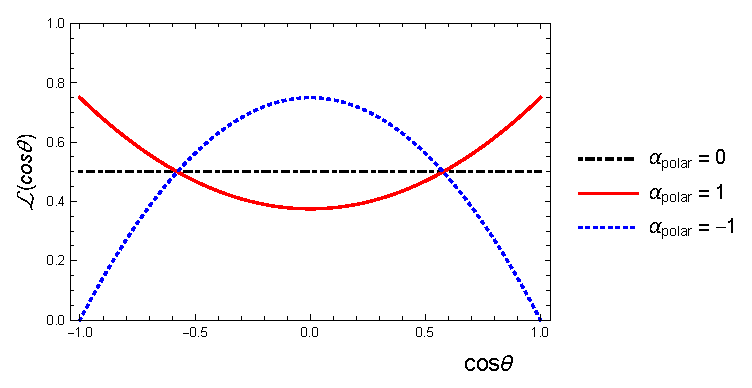
\includegraphics[width=0.9 \linewidth]{figures/angle.eps}
\caption{%
    末态赝标量粒子的极角的分布。
     黑色的虚线表示初态无极化的情况,红色的实线和蓝色的虚线分别代表只有横向极化和纵向极化的情形。
    }%
\label{fig:angle}
\end{figure}
实验家们感兴趣的是末态赝标量(或正负电子对)飞行方向的分布,我们把初态$J/\psi$的三种极化状态分布代入
公式\ref{eq:width-PVLL}之中可以得到:
\begin{equation}
\begin{split}
    & \frac{d\Gamma(\psi(\Upsilon) \to Pl^{+}l^{-}){}_{\rm{LP}}}{d\cos\theta} \sim  1- \cos^{2}\theta
    \\ & \frac{d\Gamma(\psi(\Upsilon) \to Pl^{+}l^{-}){}_{\rm{TL}}}{d\cos\theta} \sim \frac{1+ \cos^{2}\theta}{2}
    \\ & \frac{d\Gamma(\psi(\Upsilon) \to Pl^{+}l^{-}){}_{\rm{TR}}}{d\cos\theta} \sim \frac{1+ \cos^{2}\theta}{2},
\end{split}
\label{equ:angle}
\end{equation}
这里$\theta=\theta_3$即是$P$粒子在$J\psi$质心系下的极角。从而,我们可以借助于末态赝标粒子的方向信息
确定初态矢量粒子的极化状态。比如用如下的几率密度函数做拟合
\begin{equation}
     \mathcal{P}(\cos\theta) = 1 + \alpha_{\rm{polar}} \cos^{2}\theta,
\end{equation}
式中的$\alpha_{\rm polar}$用来衡量极化的大小。当$\alpha_{\rm polar} = +1$时,初态只有横向极化,
当$\alpha_{\rm{polar}} = -1$时,初态则只有纵向极化。图\ref{fig:angle}中展示了几种可能的极化状态。

\subsection{估算$\psi \to \eta_c l^{+} l^{-}$的分宽度}
从表\ref{tab:summaryresult}中列举的结果来看,衰变过程$\psi \to \eta_c l^{+} l^{-}$尚为被发现,
本小节利用公式\ref{eq:R-jpsipolar},即$\Gamma(\psi \to \eta_{c} l^{+} l^{-})$与$\Gamma(\psi \to \eta_{c} \gamma)$
的比值,来估算$\psi \to \eta_c l^{+} l^{-}$的分宽度。
过程$\psi(\Upsilon) \to P \gamma$的分宽度公式已经有文献\cite{Fu:2011yy}做了讨论,
我们直接引用其公式:
\begin{equation}
\frac{d\Gamma(\psi(\Upsilon)\to Pl^{+}l^{-})}{dq^{2}\Gamma(\psi(\Upsilon) \to P \gamma)} 
    = |F_{V\!P}(q^{2})|^{2} \times [{\rm QED}(q^{2})],
\label{equ:calVPll}
\end{equation}
式中用了正则化的形状因子$F_{V\!P}(q^{2}) \equiv
f_{V\!P}(q^{2})/f_{V\!P}(0)$,${\rm QED}(q^{2})$代表点粒子
假设下的微分宽度,即
\begin{equation}
\begin{split}
    {\rm QED}(q^{2}) = & \frac{\alpha}{3\pi} \frac{1}{q^{2}}
    \left(1-\frac{4m^{2}_{l}}{q^{2}} \right ){}^{\frac{1}{2}} \left(1 +
    \frac{2m^{2}_{l}}{q^{2}} \right)  \\ & \times \left[ \left(1 +
    \frac{q^{2}}{m^{2}_{V} - m^{2}_{P}} \right){}^{2}  -
    \frac{4m^{2}_{V}q^{2}}{(m^{2}_{V} - m^{2}_{P}){}^{2}} \right]
    {}^{\frac{3}{2}}.
\end{split}
\end{equation}
在实验上,只需要测量轻子对的能谱并与点粒子假设的理论结果做对比就能得到跃迁形状因子\cite{Landsberg:1986fd}。
由于缺少必要的实验数据,这里采取被广泛接受的VDM(vector dominance model)模型\cite{GellMann:1961tg, Bauer:1977iq},
因此在单极点近似下跃迁形状因子的形式为:
\begin{equation}
\label{fractor}
F_{V\!P}(q^{2}) = \frac{1}{1-\frac{q^{2}}{\Lambda^{2}}},
\end{equation}
这里的$\Lambda$表示一个矢量传播子的质量。
在过程$\psi \to \eta_{c} l^{+} l^{-}$中,极点的质量选取为$\psi^{\prime}$或$\psi(3770)$的质量。
我们变动极点的位置以研究衰变宽度对$\Lambda$依赖。数值计算结果表明衰变宽度对极点$\Lambda$的取值
不敏感,这很显然,因为$\Lambda$的取值远大于$q^{2}$。故我们选择$\Lambda =m_{\psi^{\prime}}$,
来计算相关的衰变宽度, 计算结果见表\ref{tab:VPll}。Fig.\ref{fig:parW}.
\begin{figure}[!htbp]
\centering
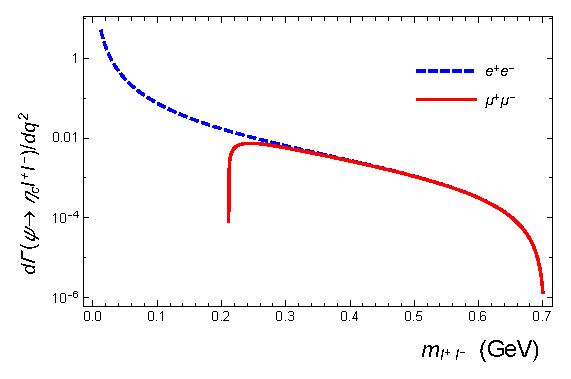
\includegraphics[width=0.9 \linewidth]{figures/partialW.eps}
\caption{过程$\psi^{\prime} \to \eta_c l^{+} l^{-}$的微分宽度。红线和蓝线分别代表$\psi^{\prime} \to \mu^+ \mu^-$
和$\psi^{\prime} \to \eta_c e^+ e^-$。}%
\label{fig:parW}
\end{figure}

\begin{table}[!htbp]
  \centering
  \caption{估计过程$\psi \to \eta_{c} l^{+} l^{-}$的分宽度。计算采取VDM模型,
    并取$\Lambda = m_{\psi^{\prime}}, m_{\psi(3770)}$ 。
    其中的误差来自于实验上$\Gamma(\psi \to \eta_{c} \gamma)$的测量结果。}%
  \label{tab:VPll}
  \begin{tabular}{p{3.5cm}p{2.5cm}<{\centering}p{2.5cm}<{\centering}}
  \toprule
   过程  &  $\Gamma^{VDM}_{ e^{+}e^{-}}$ (keV)  &  $\Gamma^{VDM}_{ \mu^{+}\mu^{-}}$ (keV) \\
  \midrule
   $J/\psi  \to \eta_{c} l^{+}  l^{-}$  &  $(9.6 \pm 2.3) \times 10^{-3}$   &  -\\
   $\psi^{\prime}  \to \eta_{c} l^{+}  l^{-}$   &  $(8.9 \pm 1.3)  \times 10^{-3}$  &  $(8.2\pm1.2) \times 10^{-4} $    \\
   %$\Upsilon({\rm{2S}}) \to \eta_{b} l^{+} l^{-}$   &  $(10.8 \pm 4.2) \times 10^{-5}$  &  $(8.2 \pm 3.2) \times 10^{-6}$    \\
   %$\Upsilon({\rm{3S}}) \to \eta_{b} l^{+} l^{-}$   &  $(9.7\pm1.6) \times 10^{-5}$  &  $(12.6\pm2.1) \times 10^{-6}$    \\
  \bottomrule
  \end{tabular}
\end{table}

\section{总结和讨论}
我们讨论了正负电子对撞机产生的$J/\psi$的极化状态,发现横向极化占主导地位,比纵向极化的强度
高出大约8个数量级。在这个结论的基础了,我们探讨了$J/\psi \to e^{+} e^{-} P$的衰变,发现极化对末态赝标量的极角影响较大,
其分布的$1+\alpha \cos^{2} \theta$,其中的$\alpha$与初态$J/\psi$的极化紧密相关,这对研究$J/\psi$极化状态
有重要的意义。同时我们预测了实验上为观测到的$\psi \to \eta_{c} e^{+} e^{-}$的宽度。
至今北京谱仪已经采集到了$10^{10}~J/\psi$和$4\times 10^{8}~\psi(2S)$样本,如果采取部分重建方法,
只重建正反电子对,并假设典型的实验效率为10\%,我们预计将分别观测到
$10^{5}$和$10^{3}$个信号。这能够精确测量分支比,甚至测量跃迁形状因子。
